% 
% ======================================================================
\RequirePackage{texmf/styles/docswitch}
% \flag is set by the user, through the makefile:
%    make note
%    make apj
% etc.
\setjournal{\flag}

\documentclass[\docopts]{\docclass}

% You could also define the document class directly
%\documentclass[]{emulateapj}

% Custom commands from LSST DESC, see texmf/styles/lsstdesc_macros.sty
\usepackage{texmf/styles/lsstdesc_macros}
\usepackage{graphics, graphicx}
\usepackage{multirow}
\graphicspath{{./}{./figures/}}
\bibliographystyle{apj}

% Add your own macros here:



% 
% ======================================================================

\begin{document}

\title{ Estimating Time Delay Measurement Feasibility in TDC2 }

\maketitlepre

\begin{abstract}

We use the 10 gateway dataset light curves and the PyCS curve-shifting analysis code to estimate time delay bias and uncertainty.

\end{abstract}

% Keywords are ignored in the LSST DESC Note style:
\dockeys{latex: templates, papers: awesome}

\maketitlepost

% ----------------------------------------------------------------------
% 

\section{Introduction}
\label{sec:intro}

In this paper, we show the analysis on the first 10 TDC2 gateway data with the use of the PyCS code.
By noticing the extra noise introduced by sampling on highly-fluctuating quasar light curve, we further introduce a new parameter $\sigma_{intrinsic}$, which rescale the noise by $\sigma_{new}=\sqrt{\sigma_{intrinsic}^2+\sigma_{old}^2}$. We also incorporate the lens model prior in our analysis.  Finally, we find that even with this crude model, we can have \textcolor{red}{more} $? \%$ success rate. 
The paper will be structured as follows.  \textcolor{red}{more}

%------------------------------------------------------------------------
\section{Method}
\label{sec:method}
In this section, we describe the process of our analysis step by step. 
\subsection{Whitening method}
The main difference between TDC2 and TDC1 data is that TDC2 tries to model the light curve taken by six different filter, which add additional variability to the light curves. We adopt the whitening method, which offsets the light curve to get a set of points that look more like they were taken in one filter. We test two kinds of whitening method. The first one (which will be called Whitening 1 hereafter) is to offset  the magnitude of whole light curves to a common mean. The second one do the same thing as the first one, but instead of offsetting all the light curves, it offset light curves season by season. Obviously, the second one (which will be called Whitening 2 hereafter)looks more reasonable because we don't expect that lightcurves in different bands have long term relations with each others. However, the second whitening will also introduced additional fluctuations to light curves, and will probably wash out the signal.  

\subsection{Additional Noise Model}
We notice that the error in the lightcurve can be larger to the reported error in TDC2 data. For example, the data in different filters will have different mean amplitude. Though the difference is partially corrected by the whitening method, it will make our light curve noisier. The micro-lensing variability could also be different for data in different filters. Besides, the light curves are sampled at an average time step 4 days, and quasars might have some high frequency fluctuation, which will also add additional noise to our light curve. 

To address this issue, we assume a simple model with only one parameter $\sigma_{intrinsic}$. The model rescales the noise in magnitude by the following formula, $\sigma_{new}=\sqrt{\sigma_{intrinsic}^2+\sigma_{old}^2}$.  Physically, it models the additional noise by a scale-free, uncorrelated log normal scatter light curve. 

\subsection{PyCS}
PyCS is a package that implements free knot spline technique described by \cite{2013A&A...553A.120T}. It models both intrinsic quasar fluctuation and also fluctuation caused by micro-lensing with two spline functions. With the use of the PyCS package, we can compute the $\chi^2$ of the fitting for a given time delay $\Delta t$. 

To analyze the data, we compute likelihood on 1000 time delay grids from -150 days to 150 days.  For each time delay, we can compute a $\chi^2$. The log likelihood function, defined as $log(P(data \mid \Delta t))$, could be computed by the following formula,
\begin{equation}
log(P(data \mid \Delta t))  = log (\Sigma_i  \frac{1}{\sqrt{2 \pi \sigma_i^2}} ) -\frac{1}{2} \chi^2,
\end{equation}
where i runs all over the data points. 

\subsection{Lens Prior}
The TDC2 data will give us an approximated fermat potential $\Delta \phi$ with some error, which can be used to compute time delay prior $P(\Delta t)$.

First, we know $P(\Delta t)$ can be calculated by the following equation.
\begin{align}
P(\Delta t) &= \int \int P(\Delta t, H_0, \Delta \phi) dH_0 d \Delta \phi \\
&= P(\Delta t | H_0, \Delta \phi) P(H_0)P(\Delta \phi) dH_0 d\Delta \phi
\end{align}

Time delay $\Delta t$ is related to the fermat potential $\Delta \phi$ by, 

\begin{equation}
\Delta t = \frac{D_{\Delta t}}{c} \Delta \phi
\end{equation}

And we know $D_{\Delta t}$ is inverse proportional to $H_0$, so we can relate $D_{\Delta t}$ to $H_0$ by the following formula, 
\begin{equation}
D_{\Delta t}= \frac{Q}{H_0}
\end{equation}
Q will be given in TDC2 data. 

From the equation $\Delta t = \frac{Q}{H_0}\Delta \phi$, where Q is a number given by the evil team, we know 
$P(\Delta t | H_0, \Delta \phi) = \delta(\Delta t - \frac{Q}{H_0}\Delta \phi)$.
Then we get
 
\begin{align}
P(\Delta t) = \int\int \delta(\Delta t - \frac{Q \Delta \phi }{H_0}) P(H_0)P(\Delta \phi) dH_0 d\Delta \phi
\end{align}

We assume $H_0$ and $\Delta \phi$ be gaussian distributions with mean $\bar{H_0}, \bar{\Delta \Phi}$ and standard deviation $\sigma_{H}$, and $\sigma_{\Delta \phi}$. 

\begin{align}
P(\Delta t) &= \frac{1}{\sqrt{2\sigma_{H}^2\pi}}\frac{1}{\sqrt{2\sigma_{\Delta \Phi}^2\pi}}\int\int \delta(\Delta t - \frac{Q \Delta \phi}{H_0}) e^{-(\frac{H_0-\bar{H_0}}{\sigma_{H}})^2} e^{-(\frac{\Delta \Phi-\bar{\Delta \Phi}}{\sigma_{\Delta \Phi}})^2} dH_0 d\Delta \phi \\
&= \frac{1}{2\sigma_{H}\sigma_{\Delta \Phi}\pi Q} exp(\frac{-\bar{H_0}^2}{\sigma_H^2}+\frac{-(\bar{\Delta \Phi})^2}{\sigma_{\Delta \Phi}^2})
exp(\frac{(\frac{\bar{H_0}}{\sigma_H^2}+\frac{\bar{\Delta \phi}\Delta t}{Q\sigma_{\Delta \phi}^2})^2}{\frac{1}{\sigma_H^2}+\frac{\Delta t^2}{\sigma_{\Delta \phi}^2 Q^2}}) \frac{\frac{\bar{H_0}}{\sigma_H^2}+\frac{\bar{\Delta \phi}\Delta t}{Q\sigma_{\Delta \phi}^2}}{\frac{1}{\sigma_H^2}+\frac{\Delta t^2}{\sigma_{\Delta\phi}^2 Q^2}}
\sqrt{\frac{\pi}{\frac{1}{\sigma_H^2}+\frac{\Delta t^2}{\sigma_\phi^2Q^2}}}
\end{align} 

If we further consider the information that the universe is expanding, which means $H_0$ is positive, the above formula will become

\begin{align}
\label{eqn:prior}
P(\Delta t) = \frac{1}{2\sigma_{H}\sigma_{\Delta \Phi}\pi Q} exp(\frac{-\bar{H_0}^2}{\sigma_H^2}+\frac{-(\bar{\Delta \Phi})^2}{\sigma_{\Delta \Phi}^2})
exp(\frac{(\frac{\bar{H_0}}{\sigma_H^2}+\frac{\bar{\Delta \phi}\Delta t}{Q\sigma_{\Delta \phi}^2})^2}{\frac{1}{\sigma_H^2}+\frac{\Delta t^2}{\sigma_{\Delta \phi}^2 Q^2}}) \frac{exp(-ab^2)+\sqrt{\pi a}b(erf(\sqrt{a}b)+1)}{2a} 
\end{align}

 where $a=\frac{1}{\sigma_H^2}+\frac{\Delta t^2}{\sigma_\phi^2Q^2}$, $b=\frac{\frac{\bar{H_0}}{\sigma_H^2}+\frac{\bar{\Delta \phi}\Delta t}{Q\sigma_{\Delta \phi}^2}}{\frac{1}{\sigma_H^2}+\frac{\Delta t^2}{\sigma_{\Delta\phi}^2 Q^2}}$, and erf is defined as $\frac{2}{\sqrt(\pi)}\int_0^z exp(-t^2) dt$

For this paper, we assume $H_0$ is $70 \pm 7$, and we compute the prior $P(\Delta t)$ by formula \ref{eqn:prior}. 

\subsection{Posterior}
The posterior can be computed by 
$P(\Delta t \mid data) = P(data \mid \Delta t) P(\Delta t)$
% ----------------------------------------------------------------------

\section{Results}
\label{sec:results}
In this section, we'll show analysis on gateway one data as an example, and we'll give a summary posterior plot for all ten gateway data. The analysis on other 9 gateway data  will be leaved to the appendix. 
\subsection{Analysis on gateway one data}
We follow the methods described in section \ref{sec:method}.  For simplicity, in this subsection, I'll only show data that is whitened by whitening method 1. 
\begin{enumerate}
\item Determine $\sigma_{intrinsic}$: 
Fig \ref{fig:sigma1} shows how likelihood change with different $\sigma_{intrinsic}$ at different time delay. First, we find that there is a clear peak at $\sigma_{intrinsic}=0.202$, and this peak does not vary at different time delays. In general, we need to compute likelihood on $\sigma_{intrinsic}$ to time delay parameter spaces. However, since the optimal $\sigma_{intrinsic}$ seems not varying for different time delay, we can find the optimal $\sigma_{intrinsic}$ at a given time delay first and then sample on time delay parameter space. 
\begin{figure}[!h]
\includegraphics[width=\textwidth, height=15cm, keepaspectratio]{sigma_0.png}
\caption{Likelihood to $\sigma_{Intrinsic}$ plot}
\label{fig:sigma1}
\end{figure}

\item Compute Prior Likelihood and Posterior:
After finding the optimal $\sigma_{intrinsic}$, we rescale the noise of light curves by $\sigma_{new}=\sqrt{\sigma_{intrinsic}^2+\sigma_{old}^2}$. Then, we compute the prior by formula \ref{eqn:prior} and likelihood with the aid of PyCS code. The prior and likelihood will be combined to get posterior. Fig \ref{fig:log_data1} shows the result.  There are couples of things to be noticed. First, the constraint on time delay is improved from prior to posterior. Second, though prior information gives us a loose constraint on time delay, it damps some of the fake peaks on likelihood and helps us identify the true time delay on posterior. For example, though there is a clear peak at true time  delay on likelihood, there are some fake outliers at  $\Delta t =140$ to $150$ and $\Delta t =-130$ to $-150$. The prior, though gives a loose constraint on time delay, damps these outliers, which helps us identified true time delay from posterior. 

\begin{figure}[!h]
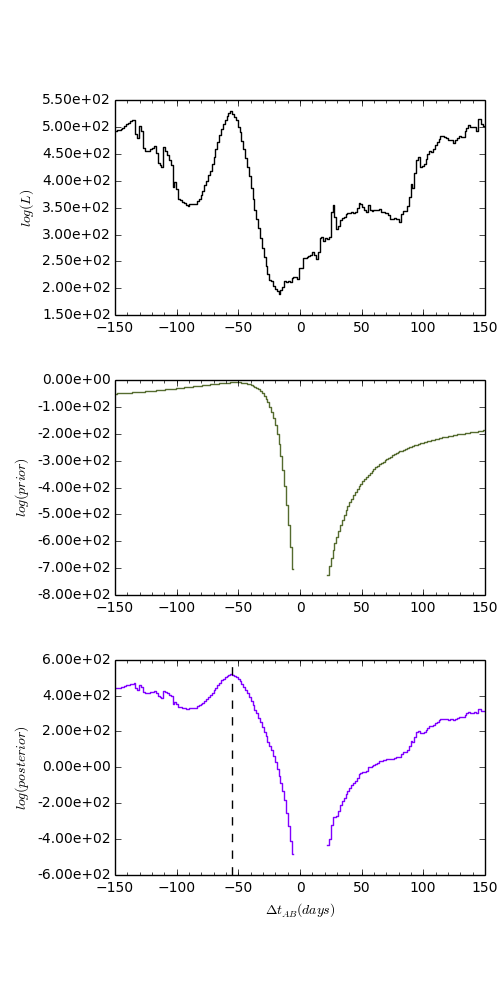
\includegraphics[width=\textwidth, height=15cm, keepaspectratio]{data1_full_log.png}
\caption{The top panel shows the likelihood distribution. The middle plot is the prior derived from equation \ref{eqn:prior}, and the bottom plot is the posterior $P(\Delta t \mid data)$ }. Dark dash line marks the correct time delay. 
\label{fig:log_data1}
\end{figure}
\end{enumerate}


\subsection{Summary of all ten gateway data sets}
Fig \ref{fig:summary_post} and fig \ref{fig:summary_prior} show the posterior and prior distributions for all 10 data, which are also summarized in Table \ref{tab:summary}.  We also compute the precision, defined as 
\begin{equation}
P=\frac{1}{N} \Sigma_i (\frac{\delta t_{i, True}}{\Delta t_i})
\end{equation}
and the accuracy
\begin{equation}
A = \frac{1}{N} \Sigma_i (\frac{\Delta t_i-\Delta t_{i, True}}{\Delta t_i}),
\end{equation}
where N is number of data, $\Delta t_i$ is the median of posterior, and $\delta t_i$ is the error of time delay, estimated by halfwidth of $68\%$ confidence region of posterior. For this ten gateway data, we reach P=0.040 and A=0.068
\begin{figure}[!h]
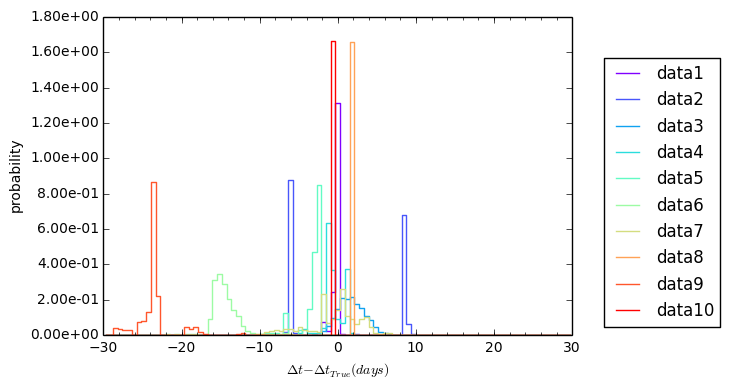
\includegraphics[width=\textwidth, height=15cm, keepaspectratio]{summary_posterior_summary.png}
\caption{}
\label{fig:summary_post}
\end{figure}

\begin{figure}[!h]
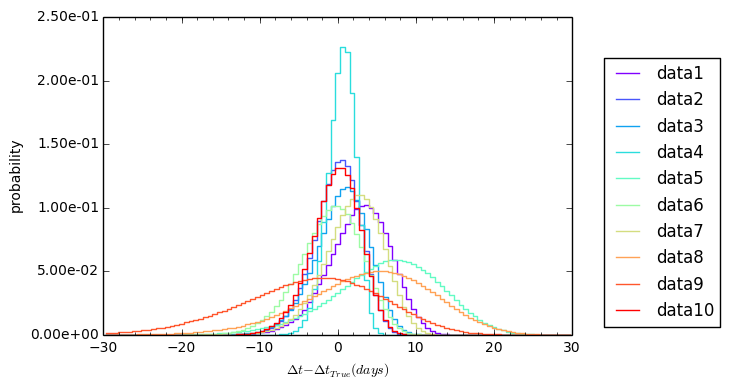
\includegraphics[width=\textwidth, height=15cm, keepaspectratio]{summary_prior_summary.png}
\caption{}
\label{fig:summary_prior}
\end{figure}

\begin{figure}[!h]
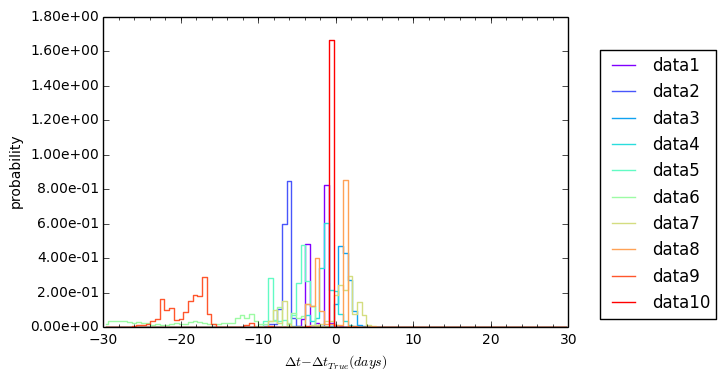
\includegraphics[width=\textwidth, height=15cm, keepaspectratio]{summary_posterior_summary_newWhiten.png}
\caption{}
\label{fig:summary_post_newWhiten}
\end{figure}



\begin{table}[]
\centering
\caption{The summary for ten gateway data analysis. $\delta \Delta t$ is the median of the difference between the measured time delay and the correct time delay. $\delta\Delta t$($68\%$) is the halfwidth of the $68\%$ credible region.}
\label{tab:summary}
\begin{tabular}{|l|l|r|l|l|l|l|}
\hline
\multicolumn{1}{|c|}{\multirow{2}{*}{data}} & \multicolumn{2}{l|}{Prior}                                                    & \multicolumn{2}{l|}{Posterior (Whitening 1)}              & \multicolumn{2}{l|}{Posterior (Whitening 2)}              \\ \cline{2-7} 
\multicolumn{1}{|c|}{}                      & $\delta\Delta t$(days) & \multicolumn{1}{l|}{$\delta\Delta t$(68$\%$) (days)} & $\delta\Delta t$ (days) & $\delta\Delta t$(68$\%$) (days) & $\delta\Delta t$ (days) & $\delta\Delta t$(68$\%$) (days) \\ \hline
1                                           & 2.97                   & 3.90                                                 & -0.34                   & 0.30                            & -1.54                   & 1.50                            \\ \hline
2                                           & -0.09                  & 2.85                                                 & -5.79                   & 7.36                            & -6.40                   & 0.30                            \\ \hline
3                                           & 0.60                   & 3.45                                                 & 1.50                    & 1.80                            & 0.90                    & 0.75                            \\ \hline
4                                           & 0.49                   & 1.65                                                 & -0.71                   & 1.35                            & -1.31                   & 0.90                            \\ \hline
5                                           & 6.65                   & 6.91                                                 & -2.96                   & 0.60                            & -4.46                   & 2.25                            \\ \hline
6                                           & -0.80                  & 4.05                                                 & -14.9                   & 1.35                            & -11.3                  & 10.8                            \\ \hline
7                                           & 1.92                   & 3.75                                                 & -0.18                   & 3.45                            & 0.72                    & 4.5                             \\ \hline
8                                           & 4.13                   & 7.96                                                 & 1.73                    & 0.15                            & 0.83                    & 2.10                            \\ \hline
9                                           & -3.18                  & 9.01                                                 & -23.9                   & 1.05                            & -18.49                  & 2.70                            \\ \hline
10                                          & -0.13                  & 3.00                                                 & -0.73                   & 0.15                            & -1.03                   & 0.15                            \\ \hline
\end{tabular}
\end{table}

\section{Discussion}
\label{sec:discussion}

If you are planning on committing your paper to GitHub, it's a good idea to write your tex as one sentence per line.
This allows for an easier \code{diff} of changes.
It also makes sense to think of latex as \emph{code}, and sentences as logical statements, occupying one line each.
Each line must ``compile'' in the mind of the reader.


% ----------------------------------------------------------------------

\section{Conclusions}
\label{sec:conclusions}

Here's a summary of what we just reported.

We can draw the following well-organized and neatly-formatted conclusions:
\begin{itemize}
  \item This is important.
  \item We can measure some number with some precision.
  \item This has some implications.
\end{itemize}

Here are some parting thoughts.


% ----------------------------------------------------------------------

\subsection*{Acknowledgments}

Here is where you should add your specific acknowledgments, remembering that some standard thanks will be added via the \code{acknowledgments.tex} file.

\input{acknowledgments}

%{\it Facilities:} \facility{LSST}

% Include both collaboration papers and external citations:
\bibliography{lsstdesc,main}

\end{document}
% ======================================================================
% 
